\documentclass[letterpaper, 10 pt, conference]{ieeeconf}  
\IEEEoverridecommandlockouts\overrideIEEEmargins
\documentclass[10pt,a4paper]{report}
\usepackage[latin1]{inputenc}
\usepackage{amsmath}
\usepackage{amsfonts}
\usepackage{amssymb}
\usepackage{graphicx}
\usepackage{tikz}
\usepackage{tabularx}
\usetikzlibrary{matrix,calc}
\usepackage[margin=0.5in]{geometry}
\usepackage{tikz}
\usetikzlibrary{arrows,shapes.gates.logic.US,shapes.gates.logic.IEC,calc}
\begin{document}
\raggedright \begin{center} 
\includegraphics[scale=0.50]{iit_h.png} \end{center}

\vspace{10mm}
\raggedright\textbf\ \hspace{1mm}\ ASSIGNMENT-1  [IDE]}  \hspace{6cm}\ Name: Dulla Srinivas\hspace{5cm} \hspace{4cm} 
roll no :\hspace{1mm} FWC22041\vspace{2cm}
\raggedright \\PROBLEM STATEMENT:\vspace{2mm}
\raggedright \\ state and Prove Commutative Law
\raggedright \\The definition of commutative law states that when we add or multiply two numbers then the resultant value remains the same, even if we change the position of the two numbers. Or we can say, the order in which we add or multiply any two real numbers does not change the result.
\vspace{1cm}
\\ sollution: A+B = B+A
 \\ \hspace{15mm}A.B = B.A
\vspace{5mm}
\\\textbf{\underline{Components:}}\vspace{2mm}
\begin{table}[ht]
\centering % used for centering table
\begin{tabular}{c c c} % centered columns (4 columns)
\hline\hline %inserts double horizontal lines
S.No & Component & Number \\ [0.5ex] % inserts table 
\hline
1 & Arduino & 1 \\
2 & Bread Board & 1 \\
3 & Jumer Wires(M-M) & 3\\
\hline
\end{tabular}
\end{table}

\vspace{5mm}
\\ \raggedright \textbf{\underline{Procedure:}}\vspace{2mm}
\\ \raggedright 1) First make the 2,3 digital pins of arduino as input pins and declare the 13 pin as output pin.
\\ 2)Write the given logic in code and upload in to the arduino.
    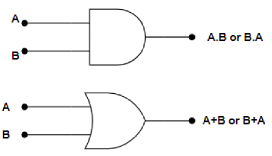
\includegraphics{pic.png}
\vspace{5cm}
\begin{figure}

    \centering
    

    \caption{Caption}
    \label{fig:my_label}
\end{figure}
\vspace{5mm}


\vspace{5cm}
\\ \raggedright \textbf{\underline{Truthtable: A+B=B+A}}\vspace{2mm}
\begin{table}[ht]
\centering % used for centering table
\begin{tabular}{c c c c c} % centered columns (4 columns)
\hline\hline %inserts double horizontal lines
 \textbf{A} & \textbf{B} & \textbf{A+B} &\textbf{B+A}\\ [0.5ex] % inserts table 
\hline
      0 & 0 & 0 & 0\\
      0 & 1 & 1 & 1\\
      1 & 0 & 1 & 1\\
      1 & 1 & 1 & 1\\
\hline
\end{tabular}
\end{table}
\vspace{2cm}
\\ \raggedright \textbf{\underline{Truthtable: A.B=B.A}}\vspace{2mm}
\begin{table}[ht]
\centering % used for centering table
\begin{tabular}{c c c c c} % centered columns (4 columns)
\hline\hline %inserts double horizontal lines
  \textbf{A} & \textbf{B} & \textbf{AB} &\textbf{BA}\\ [0.5ex] % inserts table 
\hline
      0 & 0 & 0 & 0\\
      0 & 1 & 0 & 0\\
      1 & 0 & 0 & 0\\
      1 & 1 & 1 & 1\\
\hline
\end{tabular}
\end{table}
\raggedright \textbf{\underline{}}\vspace{7mm}
\\you may  refer these code in github
\\ link    :https://github.com/Dsrinivas-sudo?tab=repositories
\vspace{2cm}
\\ #include<Ardunio.h>
\\int a;
\\int b;
\\int f;
\\int g;
\\int h;
\\int i;
\\void setup()
\\{
\\pinMode(2,INPUT);
\\pinMode(3,INPUT);
\\pinMode(13,OUTPUT);
\\pinMode(5,OUTPUT);
\\pinMode(6,OUTPUT);
\\pinMode(7,OUTPUT);
\\}
\\void loop()
\\{
\\a=digitalRead(2)
\\b=digitalRead(3)
\\f=a||b;
\\g=b||a;
\\h=a&&b;
\\i=b&&a;
\\digitalWrite(13,f);
\\digitalWrite(5,g);
\\digitalWrite(6,h);
\\digitalWrite(7,i);
\\}

\vspace{1cm}
\raggedright \textbf{\underline{Conclusion:}}\vspace{7mm}
\\ Hence have implemented the commulative law of boolean algebra in arduino and verified the outputs
\end{document}